\subsection{Space-Time Modulation}
\label{subsec:space_time_modulation}

For the case of space-time modulations, the three pairs of piezoelectric patches are driven by three equal but shifted in time signals.

The general law guiding the modulation is the following:

\begin{equation}
    Y_k^{SU} = \frac{(Y_1^D + Y_1^E)}{2} + \frac{(Y_1^D - Y_1^E)}{2} sign \left[ \cos \left( 2 \pi f_m t + (k-1) \frac{2\pi}{3} \right) \right]
\end{equation}

Where $Y_k^{SU}$ is the mechanical admittance of the $k$-th piezoelectric patch in the spatiotemporal (ST) cell, $Y_1^D$ and $Y_1^E$ are the mechanical admittance of the piezopatch in case of open and short circuit, respectively, and $f_m$ is the modulation frequency.

The phase shift between piezelectric patches imposed by the modulation $\phi=\frac{\pi}{3}$, is necessary to achieve directionality in the structure.
Thanks to this phase shift, and by properly choosing the sign of the modulation frequency, it's possible to to study both the forward and backward directionality of the wave withouth changing the excitation frequency nor it's application point.

In the following, the results of three different pairs ($\pm$) modulation frequencies are presented, and the nonreciprocal behavior of the structure is highlighted.
As for the space modulation, the experimental data are compared with the theoretical predictions obtained through the PWEM method.


\paragraph{Modulation $f_m = \pm 1 kHz$}

Forcing time modulation besides space modulation, causes dispersion diagram to becomes anti-symmetric and some of the band-gaps to be no longer global, but being localized and confined to a specific range of wavenumbers.
This is a clear indication of the nonreciprocal behavior of the structure, for which a more detailed analysis is provided in Section \ref{sec:nonreciprocal_behavior}.

Figure \ref{fig:PWEM_EXP_Sinusoidal_(discrete)_@1kHz} shows the dispersion diagram for the case of modulation frequency $f_m = \pm 1 kHz$.

\begin{figure}[H]
    \centering
    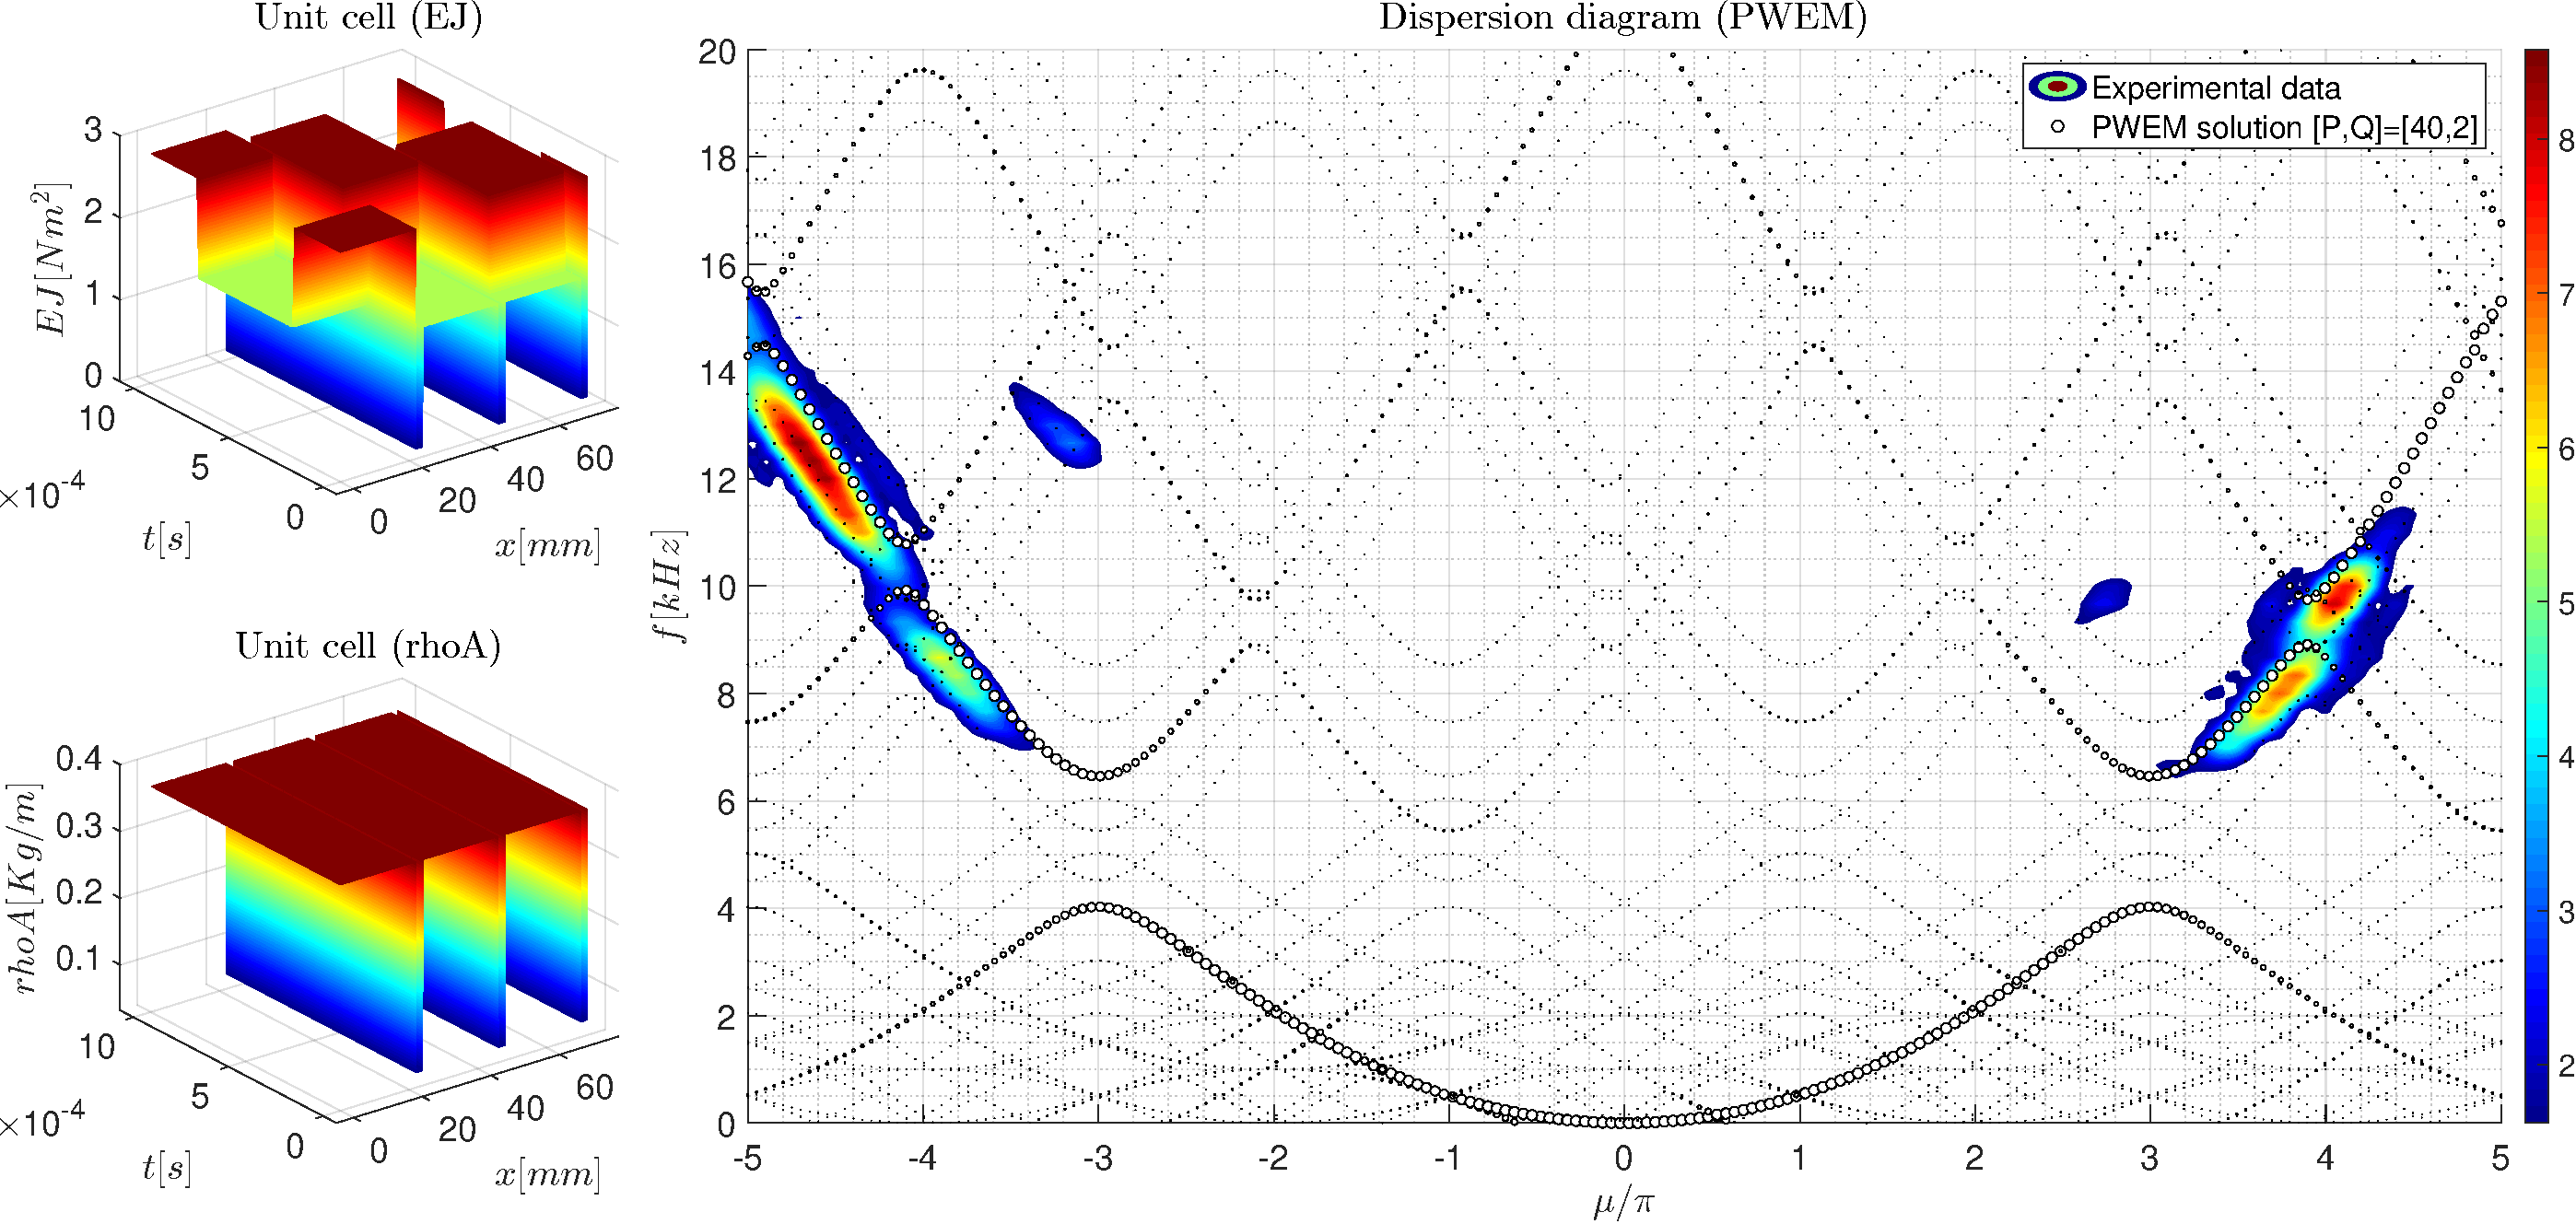
\includegraphics[width=\textwidth]{img/MATLAB/PWEM_EXP Sinusoidal (discrete) @1kHz.pdf}
    \caption{Dispersion diagram for the case of modulation frequency $f_m = \pm 1 kHz$.}
    \label{fig:PWEM_EXP_Sinusoidal_(discrete)_@1kHz}
\end{figure}

Similarly to the case of space modulation, the dispersion diagram coming from the PWEM is compared with the experimental data.
Again, except for the slight discrepancy given by the low number of harmonics considered in the PWEM, the agreement is sufficient to validate the model.

Analyzing the dispersion diagram, it's possible to observe how the first band-gap is associated with spatial modulation, while at higher frequencies nonreciprocal band-gaps associated with the time modulation appear.
In particular, it's possible to observe that at around $8.5kHz$, the first directional band-gap appears.
For the frequency range $8.5kHz < f < 9.5kHz$, we observe a band-gap for positive wavenumbers, being instead transparent in the negative wavenumber range.
On the other hand, for the frequency range $9.5kHz < f < 10.5kHz$, the band-gap is transparent for positive wavenumbers and opaque for negative wavenumbers.



\paragraph{Modulation $f_m = \pm 2 kHz$}

Similar considerations as before can be made for the case of modulation frequency $f_m = \pm 2 kHz$.

Figure \ref{fig:PWEM_EXP_Sinusoidal_(discrete)_@2kHz} shows the dispersion diagram for the case of modulation frequency $f_m = \pm 2 kHz$.

\begin{figure}[H]
    \centering
    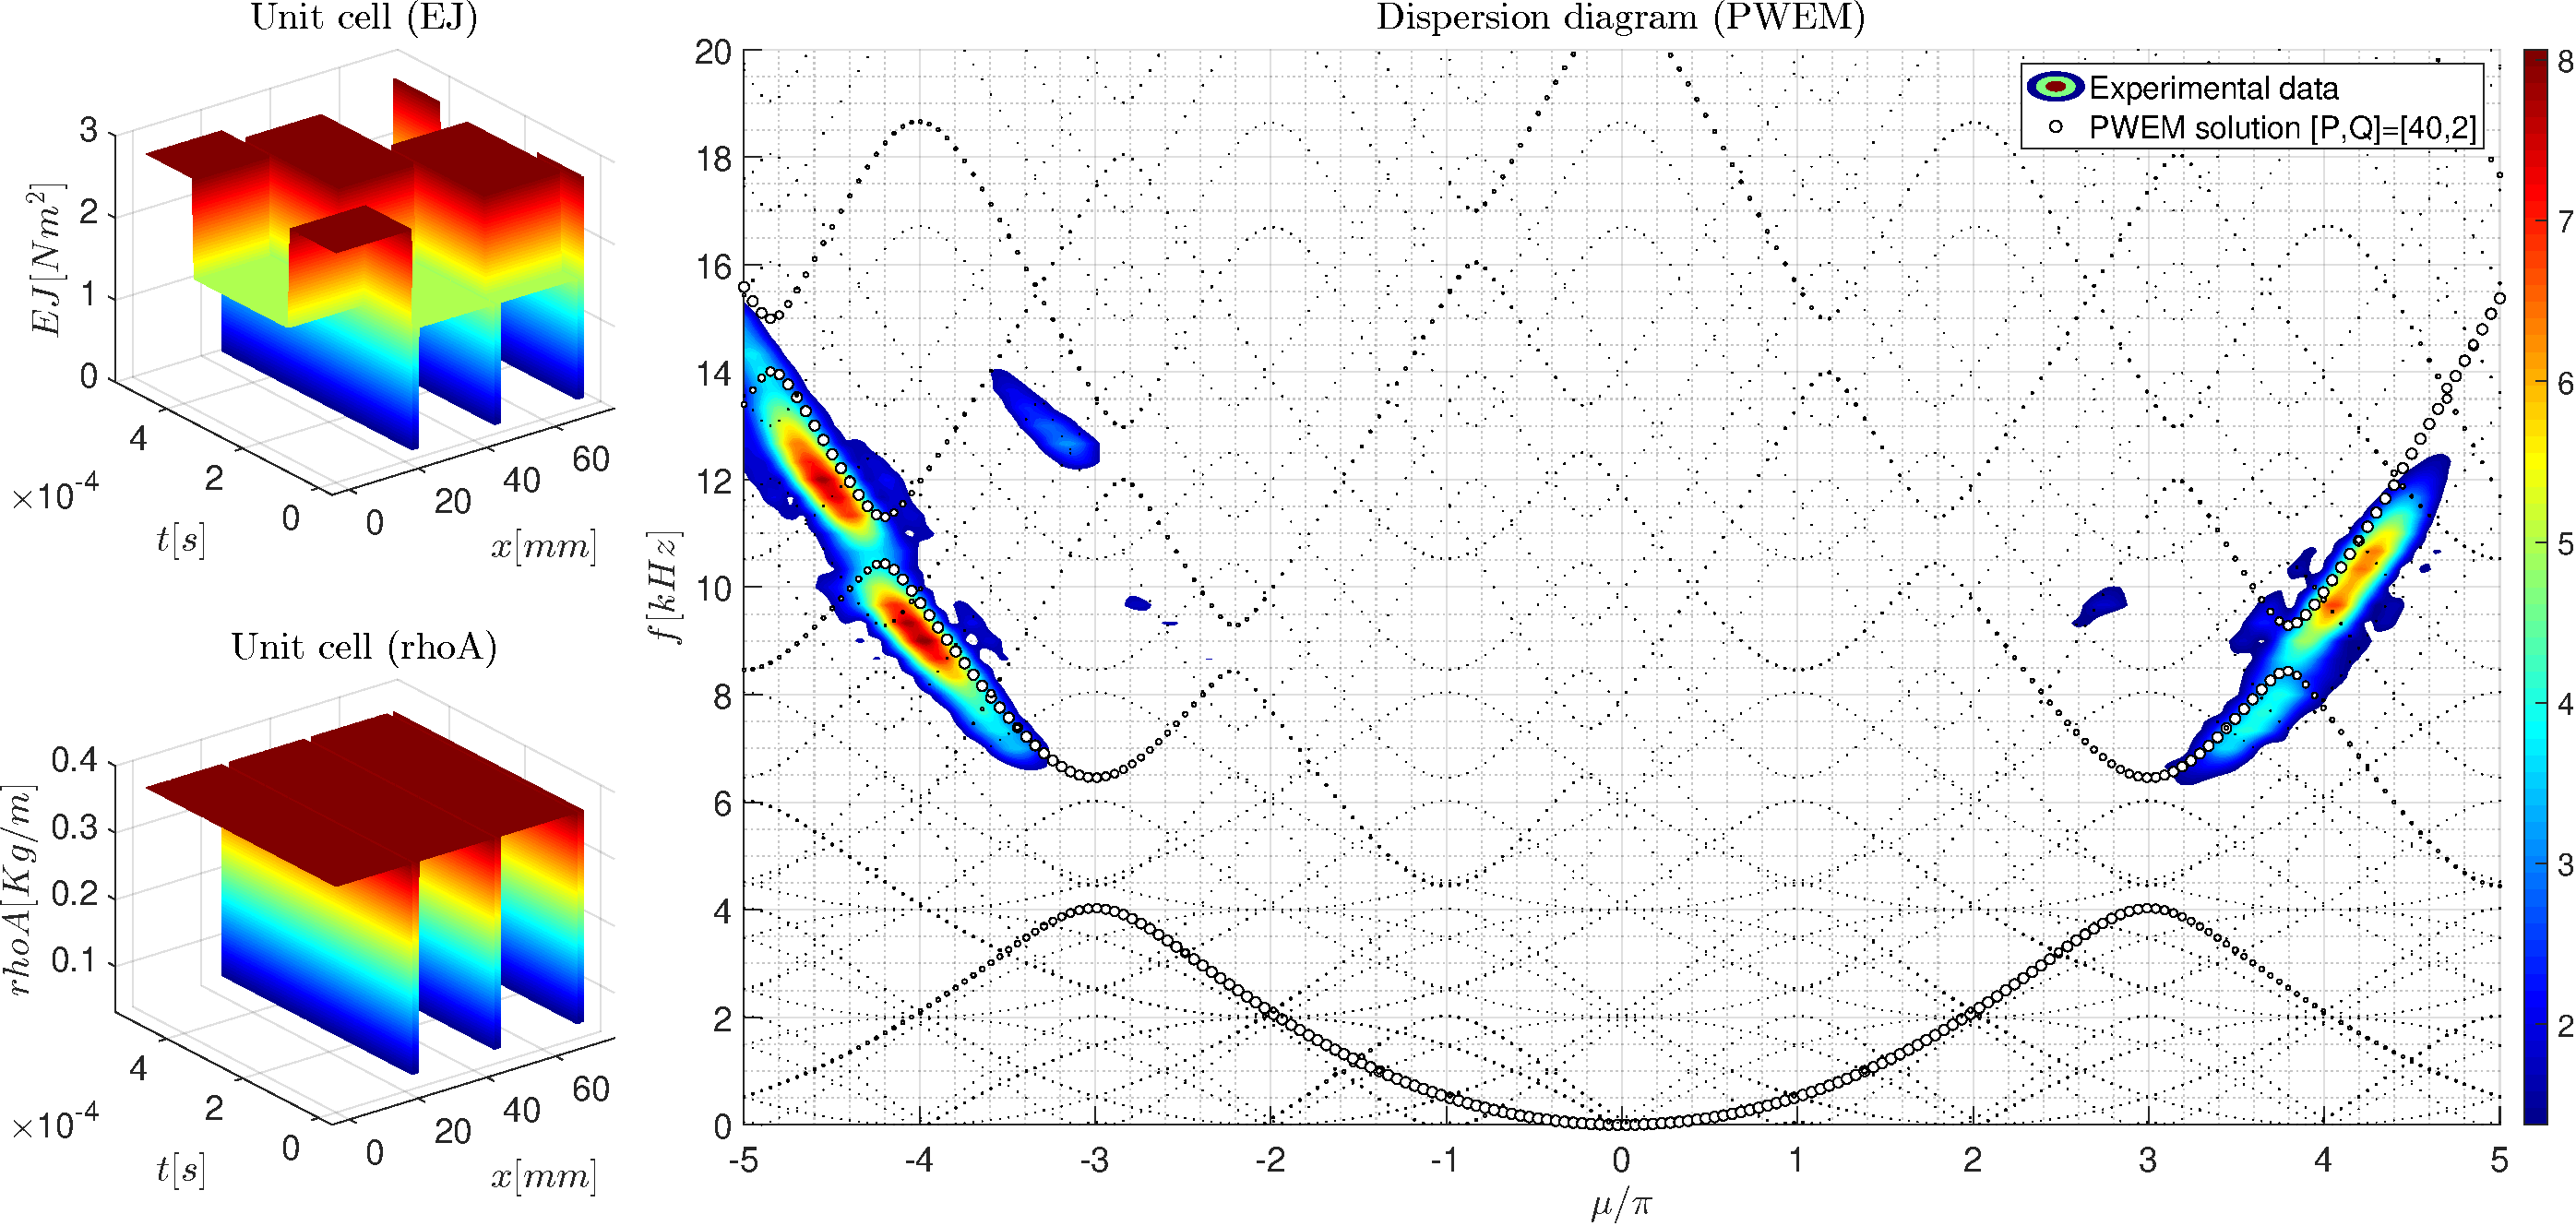
\includegraphics[width=\textwidth]{img/MATLAB/PWEM_EXP Sinusoidal (discrete) @2kHz.pdf}
    \caption{Dispersion diagram for the case of modulation frequency $f_m = \pm 2 kHz$.}
    \label{fig:PWEM_EXP_Sinusoidal_(discrete)_@2kHz}
\end{figure}

Similarly to the previous case, the dispersion diagram coming from the PWEM is compared with the experimental data.

Intuitively, the phenomenon associated with the nonreciprocal behavior is now more pronounced, as the modulation frequency is doubled.
The asymmetrical shift of the already previously analyzed directional band-gaps is even more evident.
A positive and negative shift of almost $0.5kHz$ are observed for the negative and positive wavenumbers bang-gaps, respectively.

Notice that the global band-gap at lower frequencies ($4 < f < 6.5 kHz$) is still present and hasn't been affected by the time modulation.
It's now clear that this band-gap is associated with the spatial modulation only.



\paragraph{Modulation $f_m = \pm 3 kHz$}

Figure \ref{fig:PWEM_EXP_Sinusoidal_(discrete)_@3kHz} shows the dispersion diagram for the case of modulation frequency $f_m = \pm 3 kHz$.

\begin{figure}[H]
    \centering
    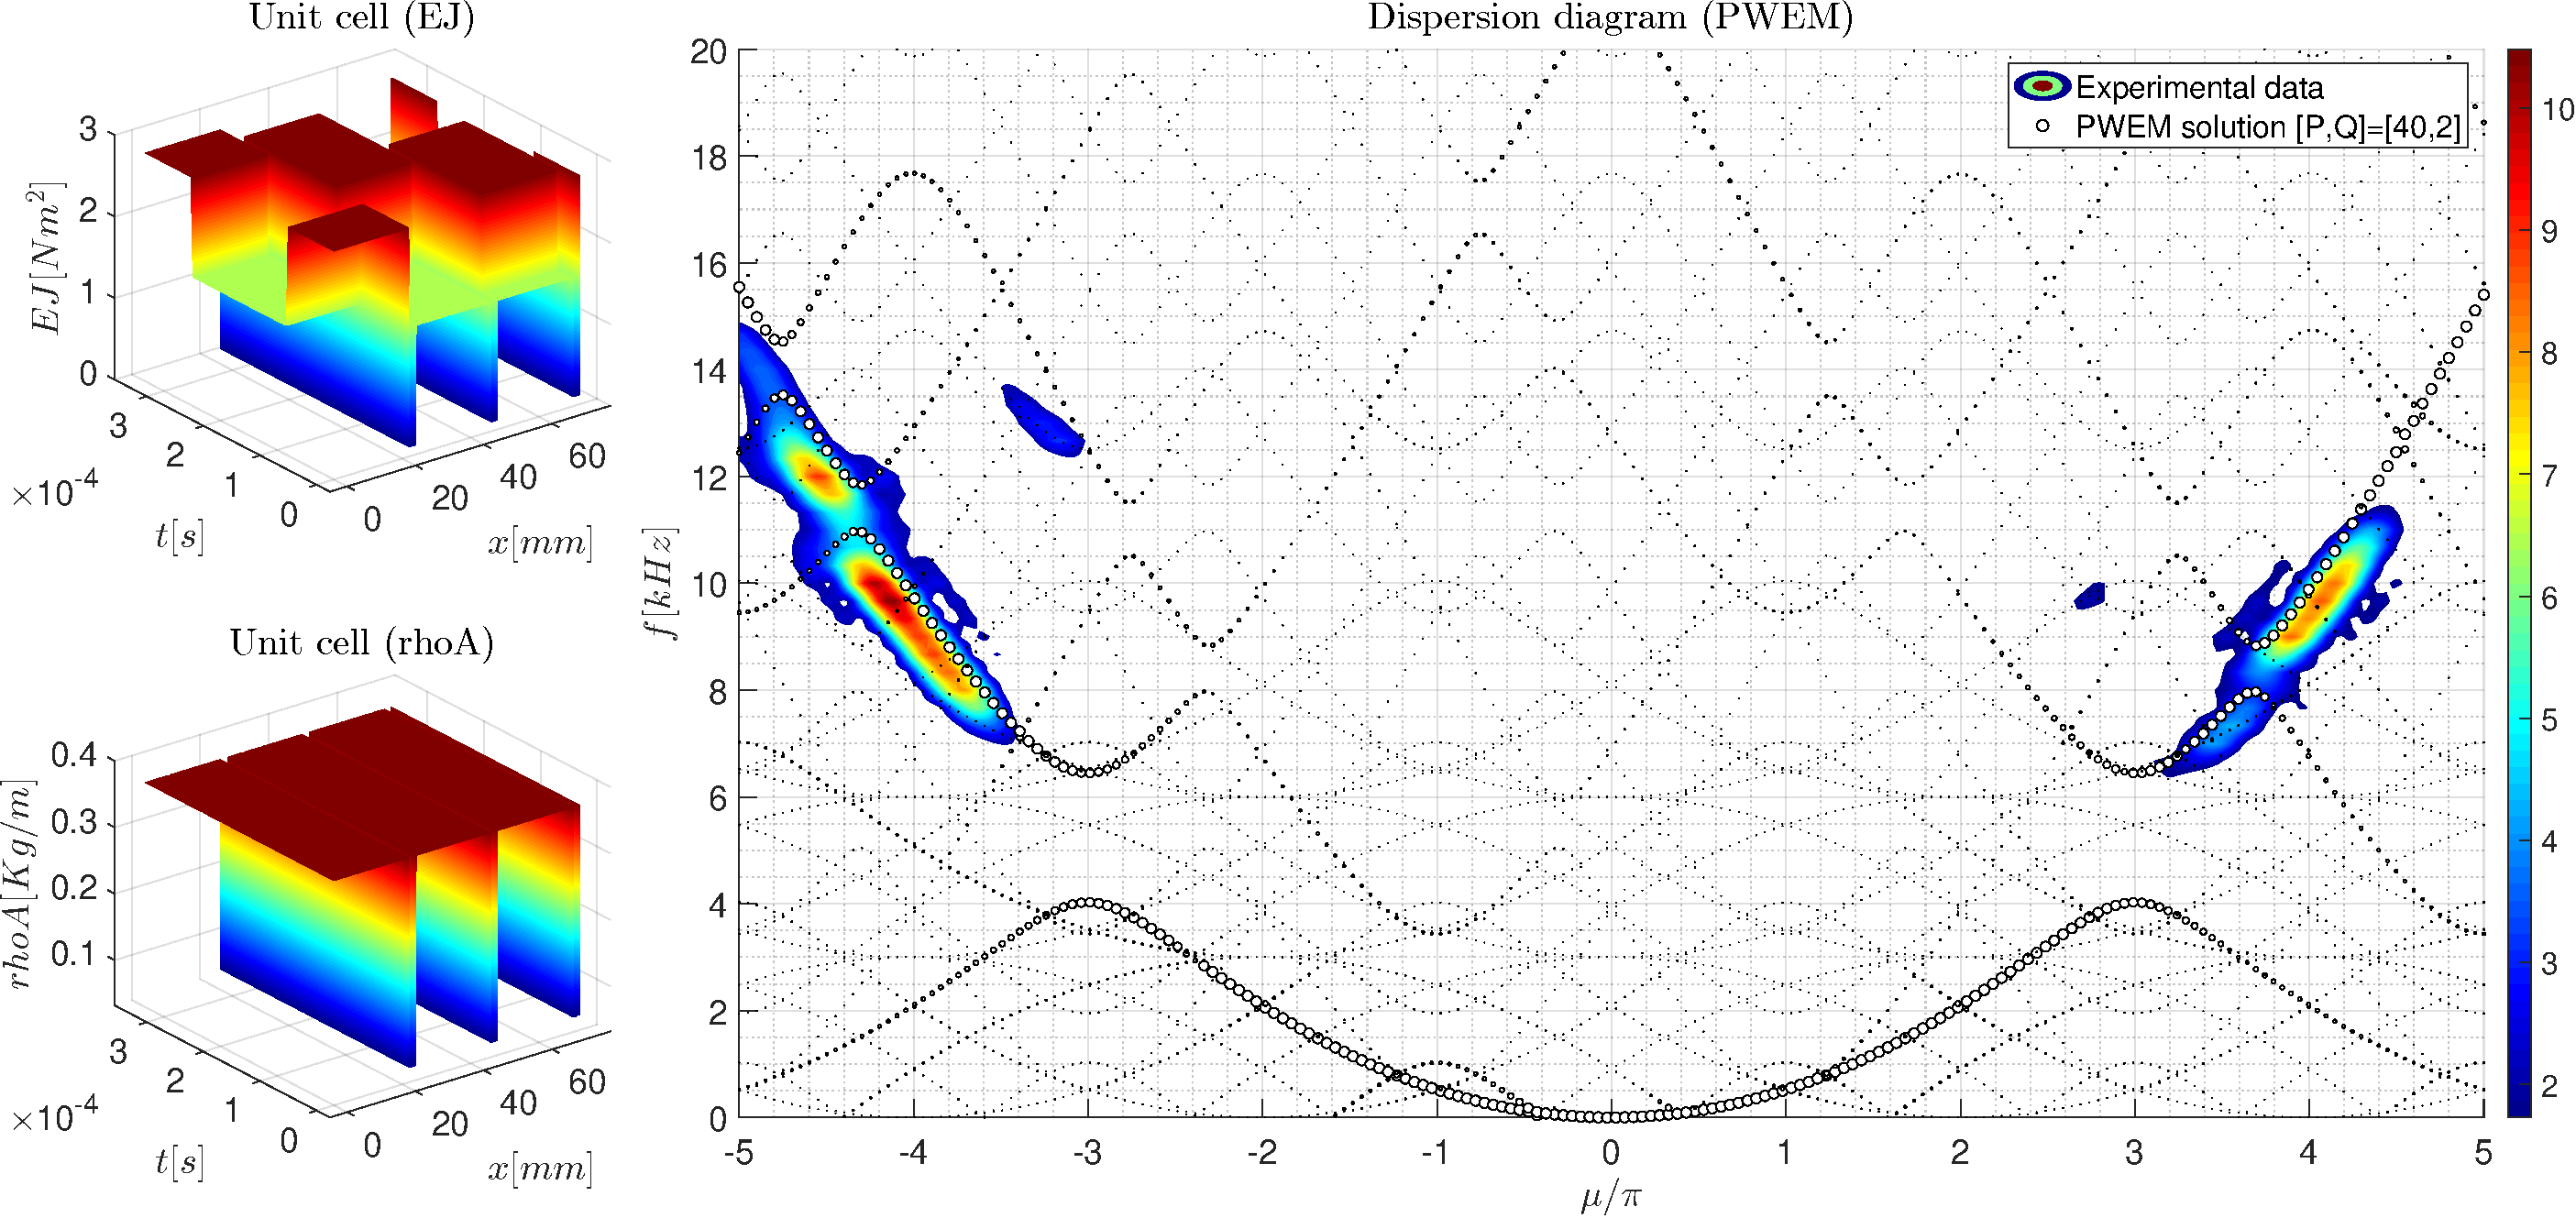
\includegraphics[width=\textwidth]{img/MATLAB/PWEM_EXP Sinusoidal (discrete) @3kHz.pdf}
    \caption{Dispersion diagram for the case of modulation frequency $f_m = \pm 3 kHz$.}
    \label{fig:PWEM_EXP_Sinusoidal_(discrete)_@3kHz}
\end{figure}

Same considerations as before can be made for the case of modulation frequency $f_m = \pm 3 kHz$.
As the modulation frequency increases, also the nonreciprocal behavior becomes more pronounced.


